%---Tracking---%
	%One point
	\input{data/tracking/qRobot1SlowTracking.txt}
	\input{data/tracking/qRobot2SlowTracking.txt}
	\input{data/tracking/qRobot3SlowTracking.txt}
	\input{data/tracking/qRobot4SlowTracking.txt}
	\input{data/tracking/qRobot5SlowTracking.txt}
	\input{data/tracking/qRobot6SlowTracking.txt}
	\input{data/tracking/qRobot7SlowTracking.txt}

	\input{data/tracking/cameraPoseP0SlowTracking.txt}
	\input{data/tracking/cameraPoseP1SlowTracking.txt}
	\input{data/tracking/cameraPoseP2SlowTracking.txt}
	\input{data/tracking/cameraPoseR0SlowTracking.txt}
	\input{data/tracking/cameraPoseR1SlowTracking.txt}
	\input{data/tracking/cameraPoseR2SlowTracking.txt}

	\input{data/tracking/errorPoseXTrackingSlow.txt}
	\input{data/tracking/errorPoseYTrackingSlow.txt}
	\input{data/tracking/errorPoseXTrackingMedium.txt}
	\input{data/tracking/errorPoseYTrackingMedium.txt}
	\input{data/tracking/errorPoseXTrackingFast.txt}
	\input{data/tracking/errorPoseYTrackingFast.txt}

	%Three Points
	\input{data/tracking/three/qRobotThreeTrackingMediumA.txt}
	\input{data/tracking/three/qRobotThreeTrackingMediumB.txt}
	\input{data/tracking/three/qRobotThreeTrackingMediumC.txt}
	\input{data/tracking/three/qRobotThreeTrackingMediumD.txt}
	\input{data/tracking/three/qRobotThreeTrackingMediumE.txt}
	\input{data/tracking/three/qRobotThreeTrackingMediumF.txt}
	\input{data/tracking/three/qRobotThreeTrackingMediumG.txt}

	\input{data/tracking/three/cameraPoseThreeTrackingMediumA.txt}
	\input{data/tracking/three/cameraPoseThreeTrackingMediumB.txt}
	\input{data/tracking/three/cameraPoseThreeTrackingMediumC.txt}
	\input{data/tracking/three/cameraPoseThreeTrackingMediumR.txt}
	\input{data/tracking/three/cameraPoseThreeTrackingMediumP.txt}
	\input{data/tracking/three/cameraPoseThreeTrackingMediumY.txt}

	\input{data/tracking/three/errorThreeTrackingSlowX.txt}
	\input{data/tracking/three/errorThreeTrackingSlowY.txt}
	\input{data/tracking/three/errorThreeTrackingMediumX.txt}
	\input{data/tracking/three/errorThreeTrackingMediumY.txt}	
	\input{data/tracking/three/errorThreeTrackingFastX.txt}
	\input{data/tracking/three/errorThreeTrackingFastY.txt}

%---Color---%
	\input{data/color/errorPoseXColorSlow.txt}
	\input{data/color/errorPoseYColorSlow.txt}

%---Corny---%



% ---------------------
% Tracking One Points
% ---------------------
\providecommand{\trackingSlowQRobotPlot}{
\begin{figure}[!ht]
	\centering
	\tikzset{every mark/.append style={scale=0.5}}
	\begin{tikzpicture}
		\begin{axis}[height=9cm, width=\textwidth, grid=major,
		xlabel={Step},ylabel={Rad}
		]	
			\addplot [color=Turquoise, mark=o] coordinates {
				\trackingSlowQRobotDataA
			};
			\addlegendentry{q1}

			\addplot [color=Orchid, mark=o] coordinates {
				\trackingSlowQRobotDataB
			};
			\addlegendentry{q2}
			
			\addplot [color=YellowGreen, mark=o] coordinates {
				\trackingSlowQRobotDataC
			};
			\addlegendentry{q3}
			
			\addplot [color=WildStrawberry, mark=o] coordinates {
				\trackingSlowQRobotDataD
			};
			\addlegendentry{q4}
			
			\addplot [color=Goldenrod, mark=o] coordinates {
				\trackingSlowQRobotDataE
			};
			\addlegendentry{q5}
			
			\addplot [color=BlueGreen, mark=o] coordinates {
				\trackingSlowQRobotDataF
			};
			\addlegendentry{q6}

			\addplot [color=CadetBlue, mark=o] coordinates {
				\trackingSlowQRobotDataG
			};
			\addlegendentry{q7}
		\end{axis}
	\end{tikzpicture}
	\caption{Robot's state while tracking the marker at slow speed.}
	\label{fig:trackingSlowQRobotPlot}
\end{figure}
}

\providecommand{\trackingSlowCameraPosePlot}{
\begin{figure}[!ht]
\centering
	\tikzset{every mark/.append style={scale=0.5}}
	\begin{tikzpicture} [spy using outlines=
	{circle, magnification=10, connect spies}
	]
		\begin{axis}[height=9cm, width=\textwidth, grid=major,
		xlabel={Step},ylabel={Rad}
		]	
			\addplot [color=Turquoise, mark=o] coordinates {
				\trackingSlowCameraPoseDataA
			};
			\addlegendentry{P0}

			\addplot [color=Orchid, mark=o] coordinates {
				\trackingSlowCameraPoseDataB
			};
			\addlegendentry{P1}
			
			\addplot [color=YellowGreen, mark=o] coordinates {
				\trackingSlowCameraPoseDataC
			};
			\addlegendentry{P2}
			
			\addplot [color=WildStrawberry, mark=o] coordinates {
				\trackingSlowCameraPoseDataD
			};
			\addlegendentry{R}
			
			\addplot [color=Goldenrod, mark=o] coordinates {
				\trackingSlowCameraPoseDataE
			};
			\addlegendentry{P}
			
			\addplot [color=BlueGreen, mark=o] coordinates {
				\trackingSlowCameraPoseDataF
			};
			\addlegendentry{Y}

			\coordinate (spypoint) at (axis cs:200,-0.31);
 			\coordinate (magnifyglass) at (axis cs:350,0.85);
		\end{axis}
		\spy [blue, size=2.0cm] on (spypoint) in node[fill=white] at (magnifyglass);
	\end{tikzpicture}
	\caption{Camera pose when tracking the marker at slow speed}
	\label{fig:trackingSlowCameraPosePlot}
\end{figure}
}

\providecommand{\trackingErrorPlot}{
\begin{figure}[!ht]
\centering
	\begin{tikzpicture}
		\begin{axis}[height=9cm, width=\textwidth, grid=major,
		xlabel={T[s]},ylabel={Pixels}
		]	
			\addplot [color=Turquoise, mark=o] coordinates {
				\TrackingSlowErrorPoseDataX
			};
			\addlegendentry{Slow Error X}

			\addplot [color=Orchid, mark=o] coordinates {
				\TrackingSlowErrorPoseDataY
			};
			\addlegendentry{Slow Error Y}
			
			\addplot [color=YellowGreen, mark=o] coordinates {
				\TrackingMediumErrorPoseDataX
			};
			\addlegendentry{Medium Error X}
			
			\addplot [color=WildStrawberry, mark=o] coordinates {
				\TrackingMediumErrorPoseDataY
			};
			\addlegendentry{Medium Error Y}
			
			\addplot [color=Goldenrod, mark=o] coordinates {
				\TrackingFastErrorPoseDataX
			};
			\addlegendentry{Fast Error X}
			
			\addplot [color=BlueGreen, mark=o] coordinates {
				\TrackingFastErrorPoseDataY
			};
			\addlegendentry{Fast Error Y}
		\end{axis}
	\end{tikzpicture}
	\caption{Error in the X and Y coordinates. Tracking marker at different speeds}
	\label{fig:trackingErrorPlot}
\end{figure}
}

% ---------------------
% Tracking Three Points
% ---------------------
\providecommand{\qRobotThreeTrackingMediumPlot}{
\begin{figure}[!ht]
	\centering
	\tikzset{every mark/.append style={scale=0.5}}
	\begin{tikzpicture}
		\begin{axis}[height=9cm, width=\textwidth, grid=major,
		xlabel={Step},ylabel={Rad}
		]	
			\addplot [color=Turquoise, mark=o] coordinates {
				\qRobotThreeTrackingMediumAData
			};
			\addlegendentry{q1}

			\addplot [color=Orchid, mark=o] coordinates {
				\qRobotThreeTrackingMediumBData
			};
			\addlegendentry{q2}
			
			\addplot [color=YellowGreen, mark=o] coordinates {
				\qRobotThreeTrackingMediumCData
			};
			\addlegendentry{q3}
			
			\addplot [color=WildStrawberry, mark=o] coordinates {
				\qRobotThreeTrackingMediumDData
			};
			\addlegendentry{q4}
			
			\addplot [color=Goldenrod, mark=o] coordinates {
				\qRobotThreeTrackingMediumEData
			};
			\addlegendentry{q5}
			
			\addplot [color=BlueGreen, mark=o] coordinates {
				\qRobotThreeTrackingMediumFData
			};
			\addlegendentry{q6}

			\addplot [color=CadetBlue, mark=o] coordinates {
				\qRobotThreeTrackingMediumGData
			};
			\addlegendentry{q7}
		\end{axis}
	\end{tikzpicture}
	\caption{Robot's state while tracking three points of the marker at medium speed.}
	\label{fig:qRobotThreeTrackingMediumPlot}
\end{figure}
}

\providecommand{\cameraPoseThreeTrackingMediumPlot}{
\begin{figure}[!ht]
\centering
	\tikzset{every mark/.append style={scale=0.5}}
	\begin{tikzpicture}
		\begin{axis}[height=9cm, width=\textwidth, grid=major,
		xlabel={Step},ylabel={Rad}
		]	
			\addplot [color=Turquoise, mark=o] coordinates {
				\cameraPoseThreeTrackingMediumAData
			};
			\addlegendentry{P0}

			\addplot [color=Orchid, mark=o] coordinates {
				\cameraPoseThreeTrackingMediumBData
			};
			\addlegendentry{P1}
			
			\addplot [color=YellowGreen, mark=o] coordinates {
				\cameraPoseThreeTrackingMediumCData
			};
			\addlegendentry{P2}
			
			\addplot [color=WildStrawberry, mark=o] coordinates {
				\cameraPoseThreeTrackingMediumRData
			};
			\addlegendentry{R}
			
			\addplot [color=Goldenrod, mark=o] coordinates {
				\cameraPoseThreeTrackingMediumPData
			};
			\addlegendentry{P}
			
			\addplot [color=BlueGreen, mark=o] coordinates {
				\cameraPoseThreeTrackingMediumYData
			};
			\addlegendentry{Y}
		\end{axis}
	\end{tikzpicture}
	\caption{Camera pose when tracking three points of the marker at medium speed.}
	\label{fig:cameraPoseThreeTrackingMediumPlot}
\end{figure}
}

\providecommand{\errorThreeTrackingPlot}{
\begin{figure}[!ht]
\centering
	\begin{tikzpicture}
		\begin{axis}[height=9cm, width=\textwidth, grid=major,
		xlabel={T[s]},ylabel={Pixels}
		]	
			\addplot [color=Turquoise, mark=o] coordinates {
				\errorThreeTrackingSlowXData
			};
			\addlegendentry{Slow Error X}

			\addplot [color=Orchid, mark=o] coordinates {
				\errorThreeTrackingSlowYData
			};
			\addlegendentry{Slow Error Y}
			
			\addplot [color=YellowGreen, mark=o] coordinates {
				\errorThreeTrackingMediumXData
			};
			\addlegendentry{Medium Error X}
			
			\addplot [color=WildStrawberry, mark=o] coordinates {
				\errorThreeTrackingMediumYData
			};
			\addlegendentry{Medium Error Y}
			
			\addplot [color=Goldenrod, mark=o] coordinates {
				\errorThreeTrackingFastXData
			};
			\addlegendentry{Fast Error X}
			
			\addplot [color=BlueGreen, mark=o] coordinates {
				\errorThreeTrackingFastYData
			};
			\addlegendentry{Fast Error Y}
		\end{axis}
	\end{tikzpicture}
	\caption{Error in the X and Y coordinates. Tracking three points of the marker at different speeds.}
	\label{fig:errorThreeTrackingPlot}
\end{figure}
}

% ---------------------
%		Color
% ---------------------
\providecommand{\colorErrorPlot}{
\begin{figure}[!ht]
\centering
	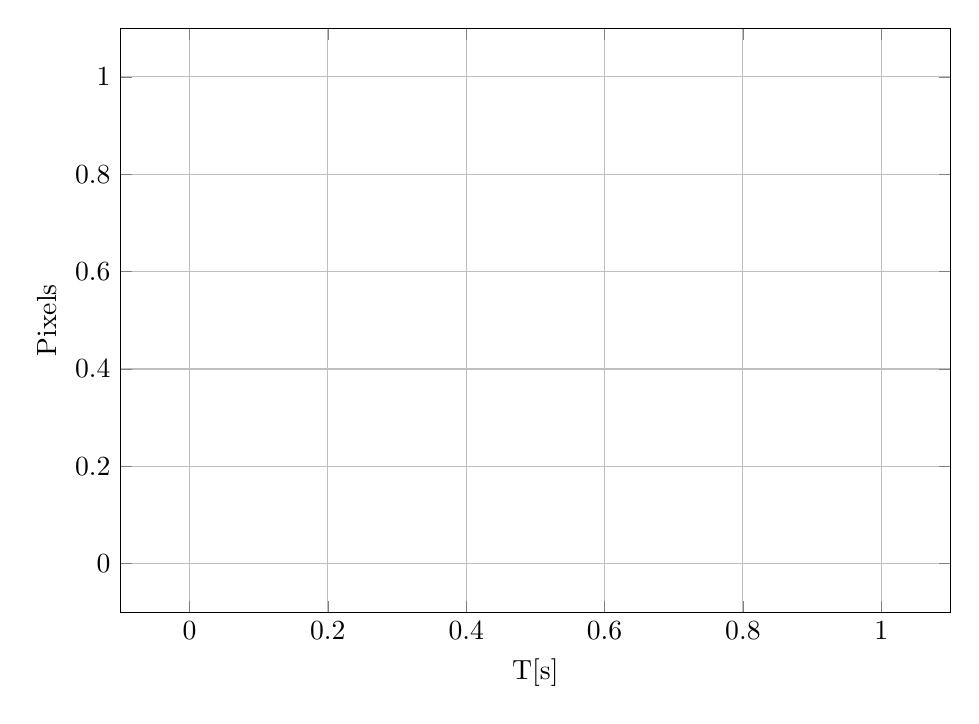
\begin{tikzpicture}
		\begin{axis}[height=9cm, width=\textwidth, grid=major,
		xlabel={T[s]},ylabel={Pixels}
		]	
			\addplot [color=Turquoise, mark=o] coordinates {
				\ColorSlowErrorPoseDataX
			};
			\addlegendentry{Slow Error X}

			\addplot [color=Orchid, mark=o] coordinates {
				\ColorSlowErrorPoseDataY
			};
			\addlegendentry{Slow Error Y}
		\end{axis}
	\end{tikzpicture}
	\caption{Error in the X and Y coordinates. Tracking marker at different speeds}
	\label{fig:colorErrorPlot}
\end{figure}
}


% ---------------------
%		Corny
% ---------------------